\documentclass{TitlePage/Configuration_Files/PoliMi3i_thesis}

\usepackage[utf8]{inputenc}
\usepackage{blindtext}
\usepackage{acronym}
\usepackage{enumitem}
\usepackage{readarray}
\usepackage{pgffor}
\usepackage{tikz}
\usepackage{float}

\def\fixcheck{%
    \def\tikzifinpicture##1##2{##2}%
}%

%Import the settings
\usepackage[a4paper]{geometry}
\usepackage[T1]{fontenc} % Extends the character set
\usepackage{fancyhdr} % Customize page layout
\usepackage{nomencl} % Nomenclature support
\usepackage[export]{adjustbox} % Elements alignment
\usepackage{graphicx} % Allows to manage images
\usepackage[sc]{mathpazo} % Math fonts
\usepackage{euler} % AMS Euler
\usepackage[detect-all]{siunitx} % Units system
\usepackage[font={footnotesize}]{caption} % Custumise captions in floating environments
\usepackage{multicol} % Enables multiple columns
\usepackage{prettyref} % Allows to specify the way in which a reference is typeset
\usepackage{pdfpages} % Used to include PDFs of more than one page
\usepackage{xargs} % Use more than one optional parameter
\usepackage{hyperref} % Hyperlinks support
\usepackage{nameref}
\usepackage{acronym} % Used in the nomenclature
\usepackage{tabularx} % Provides tables
\usepackage{longtable} % Tables spanning multiple pages
\usepackage[colorinlistoftodos]{todonotes} % TODO notes
\usepackage{xcolor}
\usepackage{wrapfig}
\usepackage[most]{tcolorbox}
\usepackage{titlesec}
\usepackage{multirow}
\usepackage{bigdelim}

\geometry{lmargin=2cm,rmargin=2cm,tmargin=2cm,marginparwidth=2cm}
\renewcommand{\headrule}{\hbox to\headwidth{\leaders\hrule height \headrulewidth\hfill}}
\renewcommand{\footrule}{\hbox to\headwidth{\leaders\hrule height \headrulewidth\hfill}}
\hypersetup{colorlinks=true, linkcolor=blue ,linktoc=page,citecolor=black}
\pagestyle{fancy}
\setcounter{secnumdepth}{3} % Set sections number depth
\setcounter{tocdepth}{3} % Table of contents depth
\setlength{\parskip}{\smallskipamount}
\setlength{\parindent}{0pt}

%Set the footer
\fancyfoot{}
\fancyfoot[L]{\fontsize{9}{11} \selectfont DD Project}
\fancyfoot[R]{\fontsize{9}{11} \selectfont \thepage}

%Set the top layout
\fancyhead{} % Clear all header fields
\pagestyle{fancyplain} % Defines a new header for all pages
%\fancyheadoffset[]{0.2pt}
\lhead{
    \raisebox{-0.35cm}{
        
\includegraphics[height=1.2cm,keepaspectratio]{polimi-logo.png}
    }
}

\tikzset{
    ->, % makes the edges directed
    node distance=3cm, % specifies the minimum distance between two nodes. Change if necessary.
    every state/.style={thick, fill=gray!10}, % sets the properties for each ’state’ node
}

\rhead{\rule[-2ex]{0pt}{2ex}\fontsize{9}{11} \selectfont Politecnico di Milano}

\setlength{\headheight}{38.68459pt}

% CONFIGURATIONS
\usepackage{parskip} % For paragraph layout
\usepackage{setspace} % For using single or double spacing
\usepackage{emptypage} % To insert empty pages
\usepackage{multicol} % To write in multiple columns (executive summary)
\setlength\columnsep{15pt} % Column separation in executive summary
\setlength\parindent{0pt} % Indentation
\raggedbottom  

% PACKAGES FOR TITLES
\usepackage{titlesec}
% \titlespacing{\section}{left spacing}{before spacing}{after spacing}
\titlespacing{\section}{0pt}{3.3ex}{2ex}
\titlespacing{\subsection}{0pt}{3.3ex}{1.65ex}
\titlespacing{\subsubsection}{0pt}{3.3ex}{1ex}
\usepackage{color}

% PACKAGES FOR LANGUAGE AND FONT
\usepackage[english]{babel} % The document is in English  
\usepackage[utf8]{inputenc} % UTF8 encoding
\usepackage[T1]{fontenc} % Font encoding
\usepackage[11pt]{moresize} % Big fonts

% PACKAGES FOR IMAGES
\usepackage{graphicx}
\usepackage{transparent} % Enables transparent images
\usepackage{eso-pic} % For the background picture on the title page
\usepackage{subfig} % Numbered and caption subfigures using \subfloat.
\usepackage{tikz} % A package for high-quality hand-made figures.
\usetikzlibrary{}
\graphicspath{{./Images/}} % Directory of the images
\usepackage{caption} % Coloured captions
\usepackage{xcolor} % Coloured captions
\usepackage{amsthm,thmtools,xcolor} % Coloured "Theorem"
\usepackage{float}

% STANDARD MATH PACKAGES
\usepackage{amsmath}
\usepackage{amsthm}
\usepackage{amssymb}
\usepackage{amsfonts}
\usepackage{bm}
\usepackage[overload]{empheq} % For braced-style systems of equations.
\usepackage{fix-cm} % To override original LaTeX restrictions on sizes

% PACKAGES FOR TABLES
\usepackage{tabularx}
\usepackage{longtable} % Tables that can span several pages
\usepackage{colortbl}

% PACKAGES FOR ALGORITHMS (PSEUDO-CODE)
\usepackage{algorithm}
\usepackage{algorithmic}

% OTHER PACKAGES
\usepackage{pdfpages} % To include a pdf file
\usepackage{afterpage}
\usepackage{lipsum} % DUMMY PACKAGE
\usepackage{fancyhdr} % For the headers
\fancyhf{}

% Input of configuration file. Do not change config.tex file unless you really know what you are doing. 
% Define blue color typical of polimi
\definecolor{bluepoli}{cmyk}{0.4,0.1,0,0.4}

% Custom theorem environments
\declaretheoremstyle[
  headfont=\color{bluepoli}\normalfont\bfseries,
  bodyfont=\color{black}\normalfont\itshape,
]{colored}

% Enhances the features of the standard "table" and "tabular" environments.
\newcommand\T{\rule{0pt}{2.6ex}}
\newcommand\B{\rule[-1.2ex]{0pt}{0pt}}

% Pseudo-code algorithm descriptions.
\newcounter{algsubstate}
\renewcommand{\thealgsubstate}{\alph{algsubstate}}
\newenvironment{algsubstates}
  {\setcounter{algsubstate}{0}%
   \renewcommand{\STATE}{%
     \stepcounter{algsubstate}%
     \Statex {\small\thealgsubstate:}\space}}
  {}

% New font size
\newcommand\numfontsize{\@setfontsize\Huge{200}{60}}

% Title format: section
\titleformat{\section}
{\color{bluepoli}\normalfont\Large\bfseries}
{\color{bluepoli}\thesection.}{1em}{}

% Title format: subsection
\titleformat{\subsection}
{\color{bluepoli}\normalfont\large\bfseries}
{\color{bluepoli}\thesubsection.}{1em}{}

% Title format: subsubsection
\titleformat{\subsubsection}
{\color{bluepoli}\normalfont\large\bfseries}
{\color{bluepoli}\thesubsubsection.}{1em}{}

% Shortening for setting no horizontal-spacing
\newcommand{\hsp}{\hspace{0pt}}

\makeatletter
% Renewcommand: cleardoublepage including the background pic
\renewcommand*\cleardoublepage{%
  \clearpage\if@twoside\ifodd\c@page\else
  \null
  \AddToShipoutPicture*{\BackgroundPic}
  \thispagestyle{empty}%
  \newpage
  \if@twocolumn\hbox{}\newpage\fi\fi\fi}
\makeatother


%----------------------------------------------------------------------------
%	NEW COMMANDS DEFINED
%----------------------------------------------------------------------------

% EXAMPLES OF NEW COMMANDS
\newcommand{\bea}{\begin{eqnarray}} % Shortcut for equation arrays
\newcommand{\eea}{\end{eqnarray}}
\newcommand{\e}[1]{\times 10^{#1}}  % Powers of 10 notation


\usepackage[acronym]{glossaries}

\makenoidxglossaries%

\newglossaryentry{partita IVA}{
    name={partita IVA},
    description={Outside the Italian territory it corresponds to the VAT number. It is a unique identifier for the operators that want to perform an economical activity in the national territory}
}



\begin{document}
\fancypagestyle{plain}{%
\fancyhf{} % Clear all header and footer fields
\fancyhead[RO,RE]{\thepage} %RO=right odd, RE=right even
\renewcommand{\headrulewidth}{0pt}
\renewcommand{\footrulewidth}{0pt}}

%----------------------------------------------------------------------------
%	TITLE PAGE
%----------------------------------------------------------------------------
\thispagestyle{empty}%
% \frontmatter % Use roman page numbering style (i, ii, iii, iv...) for the preamble pages

\puttitle{
	title=RASD - Software Engineering 2, % Title of the thesis
	name={\\ \bfseries{Emilio Corigliano (10627041)}\\ \bfseries{Federico Mandelli (10611353)}\\ \bfseries{Matteo Pignataro (10667498)}}, % Author Name and Surname
	course=Computer Science and Engineering, % Study Programme (in Italian)
	advisor= Prof. Matteo Camilli, % Supervisor name
	coadvisor={Prof.ssa Elisabetta Di Nitto, Prof. Matteo Giovanni Rossi}, % Co-Supervisor name, remove this line if there is none
	academicyear={2022-23},  % Academic Year
} % These info will be put into your Title page 

%----------------------------------------------------------------------------
%	PREAMBLE PAGES: ABSTRACT (inglese e italiano), EXECUTIVE SUMMARY
%----------------------------------------------------------------------------
% \startpreamble
\clearpage

%Index
\tableofcontents{}
\clearpage

%Introduction
\section{Introduction}

% \ac{} Stampa l'acronimo completo solo la prima volta che lo si usa e in parentesi l'acronimo;
% \acf{} Stampa sempre l'acronimo completo e in parentesi l'acronimo;
% \acp{} Come \ac ma aggiunge la s alla fine per il plurale;
% \acl{} Stampa solo l'acronimo completo.

% Introduction
\todo[inline]{
    - Aggiungere nei world phenomena il ChargingType\\
    - Inserire "vehicle type" all'interno dell'attore auto (Ho messo consumption per Km perchè altrimenti avremmo dovuto definire una sorta di lista di tipi di macchine)\\
    - Controlla che gli Scenarios siano coerenti con l'UML\\
    - Aggiorna Requirements con spiegazione di EnergySourceStrategy\\
    - Update Scenarios with "Giochini di Emilio"
    - Better explain in Requirements(not sure) how the system suggest a charge
}

\subsection{Purpose}
Due to the recently increase of effort in the battle against the climate change, electric vehicles are slowly becoming the new technology for private transport that the people use everyday.
To sustain this type of strategy, we need to develop a clever and capillary charging system.\\
\ac{eMall} is an \ac{eMSP} that aims to help the final user dealing with the charging need.
To do so it will inform the user about the nearby charging stations, their cost and any special offer that they have.
Also, it will allow the user to book/cancel/pay a charge and will notify the user when the charging process is terminated.
With the integration of the user's calendar, the system will also suggest the user the best moment in the schedule to charge the vehicle.
To have a fully integrated system, all the \acp{CPO} will have a technological support called \ac{CPMS} to interface the service with the physical charging stations and to manage all the energy sources like batteries and \acp{DSO}.
Such \acp{CPMS} will be in charge of deciding the energy source and, in case of batteries in a charging station it will also manage their charging.
These decisions will affect the energy prices, so it is important that a system like this allows also the \ac{CPO} maintainers to decide it.
\subsubsection{Goals}
%\input{Introduzione}
\begin{enumerate}[label=\textbf{G\arabic*}]
    \item The \ac{eMSP} shall help the user to select the station; \label{goal:eMSP-helps-selecting}
    \item The \ac{eMSP} shall allow the user to book/cancel a charge; \label{goal:eMSP-booking-charge}
    \item The \ac{eMSP} shall allow the user to perform a charge; \label{goal:eMSP-allow-charge}
    \item \acp{CPMS} shall handle the vehicle charging cycles; \label{goal:CPMS-handles-charge}
    \item \acp{CPMS} shall manage the vehicle charging stations; \label{goal:CPMS-manage-station}
\end{enumerate}

% Subsection where we enumerate all the world and shared phenomena
\subsection{Scope}

% world phenomena
\begin{enumerate}[label=\textbf{W\arabic*}]
    \item People charge electric vehicles; \label{world:people-charge-vehicles} [\ref{goal:eMSP-helps-selecting}, \ref{goal:eMSP-booking-charge}, \ref{goal:eMSP-allow-charge}, \ref{goal:CPMS-handles-charge}]
    \item People use web calendar; \label{world:people-use-calendars} [\ref{goal:eMSP-helps-selecting}, \ref{goal:eMSP-booking-charge}, \ref{goal:eMSP-allow-charge}]
    \item People pay for the charging service; \label{world:people-pay-service} [\ref{goal:eMSP-allow-charge}]
    \item \acp{DSO} supply energy to \acp{CPO}; \label{world:DSO-supply-energy} [\ref{goal:CPMS-manage-station}]
    \item Some \acp{CPO} own batteries; \label{world:CPO-own-batteries} [\ref{goal:CPMS-handles-charge}, \ref{goal:CPMS-manage-station}]
    \item \acp{CPO} decide whether to use batteries or \ac{DSO} supplied energy; \label{world:CPO-decide-energy} [\ref{goal:CPMS-handles-charge}, \ref{goal:CPMS-manage-station}]
\end{enumerate}
% shared phenomena
\begin{enumerate}[label=\textbf{S\arabic*}]
    % system -> user
    \item The \ac{eMSP} suggests the user to charge the vehicle; \label{shared:eMSP-suggests-charge} [\ref{goal:eMSP-helps-selecting}]
    \item The \ac{eMSP} notifies the user when the charging process is finished; \label{shared:eMSP-notifies-charging-finished} [\ref{goal:eMSP-allow-charge}]
    \item \acp{CPMS} acquire information about energy prizes from \acp{DSO}; \label{shared:CPMS-info-from-DSO} [\ref{goal:CPMS-manage-station}]
          % user -> system
    \item The user books a charge using the \ac{eMSP}; \label{shared:user-books-charge} [\ref{goal:eMSP-booking-charge}]
    \item The user asks the \ac{eMSP} for suggestions about charging station; \label{shared:user-asks-suggestions} [\ref{goal:eMSP-helps-selecting}]
    \item The user pays for the service using the \ac{eMSP}; \label{shared:user-pays-service} [\ref{goal:eMSP-allow-charge}]
    \item \acp{CPO} gather the energy source through the \ac{CPMS}; \label{shared:CPO-energy-through-CPMS} [\ref{goal:CPMS-handles-charge}, \ref{goal:CPMS-manage-station}]
\end{enumerate}

\subsection{Definitions, Acronyms, Abbreviations}
\begin{multicols}{2}[]
    \begin{acronym}[RASD]
        \acro{eMSP}{e-Mobility Service Providers}
        \acro{CPO}{Charging Point Operators}
        \acro{CPMS}{Charge Point Management System}
        \acro{DSO}{Distribution System Operators}
        \acro{eMall}{e-Mobility for All}
        \acro{API}{Application Programming Interface}
    \end{acronym}
\end{multicols}

\subsection{Revision history}

\subsection{Reference Documents}

\subsection{Document Structure}

% \def\goalsToPhenomena{
% {1,2}, 
% {3,4}}

% \foreach \g in \goalsToPhenomena{
%     \pgfmathparse{{\g}[0]}\pgfmathresult : \pgfmathparse{{\g}[1]}\pgfmathresult

% }
\clearpage

% General description about the system
\section{Overall Description}
\subsection{Product perspective}

\subsubsection{Scenarios}
It is assumed that in S4,S5,S6,S7 the user is already logged in the system (S2)
\begin{enumerate}[label=\textbf{S\arabic*}]
      \item User Signs up:\\
            Lucy, wanting to use the system, opens the app, she is prompted to login or register,
            she chooses to register herself and inserts her personal info (email, password, birthday, payment information, vehicle info);
            an email is sent with a link to confirm the activation of the account, if the link is clicked within
            the first 15 minutes the account is activated and the sign up is successful,
            otherwise it is considered failed and the process must be repeated.
      \item User Logs in:\\
            Jay, after signing up, opens the app and he is prompted to insert his email and password,
            if the given information are correct the login is successful and he obtain access to his account
            and the services of the app, otherwise the login is unsuccessful and it must be repeated.
      \item User searches for stations:\\
            Robert, once logged in, inserts the location and the time frame to search for charging stations.
            Once submitted, a list of available charging stations is displayed, the list is ordered by the distance of the station
            from the desired location. Via a menu, Robert can choose to order the stations either via distance, price or charging type (super-fast, fast, normal); He can also set to display unavailable stations and set the maximum distance from the chosen location.
            Robert chooses a station and obtains more detailed information.
      \item User books a charge:\\
            Jessica, after choosing a station, decides to book a charge in it selecting the timeslot. Station location and booked time frame are displayed and she is asked to confirm the booking via a popup. She receives a confirmation email with the details
            of the charge (Location, time frame, socket id) and a confirmation pin to insert at the station.
      \item User pays a charge:\\
            John, after booking a charge, has to pay it before actually performing it. So he selects the wanted charge and proceeds with the payment. After that he receives an email that summarizes the payment details.
      \item User cancels a charge:\\
            Luke, after booking a charge, wants to cancel it. He opens the app, selects the booking he wants to cancel and presses the Cancel button. A popup appear asking confirmation: if it is pressed the booking is removed, the station returns available, a refound is issued and a confirmation email is sent to the user; otherwise the booking is still valid.
      \item User charges the vehicle:\\
            Mary, after booking a charge, arrives at the station, she parks her vehicle at the designed socket
            and plugs her vehicle in, Mary then inserts the confirmation pin in the socket to start the charge.
            The socket displays on a monitor the status and the finishing time of the charge.
            Once the charge is finished Mary receives a notification of finished charge,
            she gets her vehicle and completes the charge.
      \item User gets charging suggestion based on his calendar:\\
            Josh is a very busy man and also an avid google calendar user,
            setting up every event with correct time and location.
            The service accessing his calendar finds the closest available charging station to each vehicle movement,
            it connects to the vehicle while driving and stores the last charge level and once the battery is below fifty percent Josh gets notified
            about the possibility to charge his vehicle in an available time-slot and near his movement.
            Josh liking the idea opens the app and confirms the booking.
      \item Cpo adds stations to the CPMS:\\
            Frank, the responsible for a CPO, wants to add stations to the CPMS in preparation of subscribing to eMall. For each station he has to insert the number of charging port, the presence of batteries and, if there are any, the \ac{API} reference,
            wether to use the CPMS automatic source selector or to choose the preferred energy source.
      \item Cpo subscribes to the system:\\
            Judy, the CEO of a famous CPO, wants to subscribe it to eMAll to improve sales.
            She opens the eMall website and selects to sign up, she inserts the name, partita iva, a master password and connects the CPMS of to the site via an \ac{API}.
      \item Cpo updates info about its system:\\
            The sysadmin of a CPO, Andy, after logging in with the master password has access to his CPMS.
            \todo{Data la presenza di \ac{API} per le charging stations, deve per forza inserire queste info?}
            Here he can change the number of stations, for each station he can update the number of sockets and the energy source.
            He can also create and update maintainer account inserting the ID and password. For each maintainer he can choose which CPMS the maintainer can maintain.
      \item Cpo employee logs in the service:\\
            Brett a CPO employee wants to access the service, he connects to the site and inserts the ID
            \todo{Quale sito?}
            and password, if correct he logs in; otherwise the procedure fails and must be repeated.
      \item Maintainer maintains his assigned CPMS\\
            Lisa, a maintainer at a cpo logs in the service, here she can see the info of each station of the CPMS assigned to her.
            For each station she can: check the status(functioning or not), choose the energy source, update the number of available sockets.
            She can monitor the consumes, profitability and the usage of a specified station.
\end{enumerate}

\clearpage
\todo[inline]{- Il CPO registra il suo servizio nel eMSP convalidato da partita IVA\\
      - Il CPO indica all'eMSP l'accesso all'interfaccia del suo/dei suoi CPMS\\
      - L'eMSP contatta l'interfaccia del/dei CPMS per ottenere info sulle charging stations\\
      - L'utente paga PRIMA della recharge in base alle info del veicolo e solo dopo il pagamento gli viene assegnato un codice di ricarica che l'eMSP comunica al CPMS che lo comunica alla chargingStation che lo accetta per ricarica\\
      - In caso di cancellazione viene effettuato rimborso\\
      MODIFICARE L'UML DI CONSEGUENZA}
\subsubsection{UML diagram}
\begin{figure}[h!]
      \begin{center}
            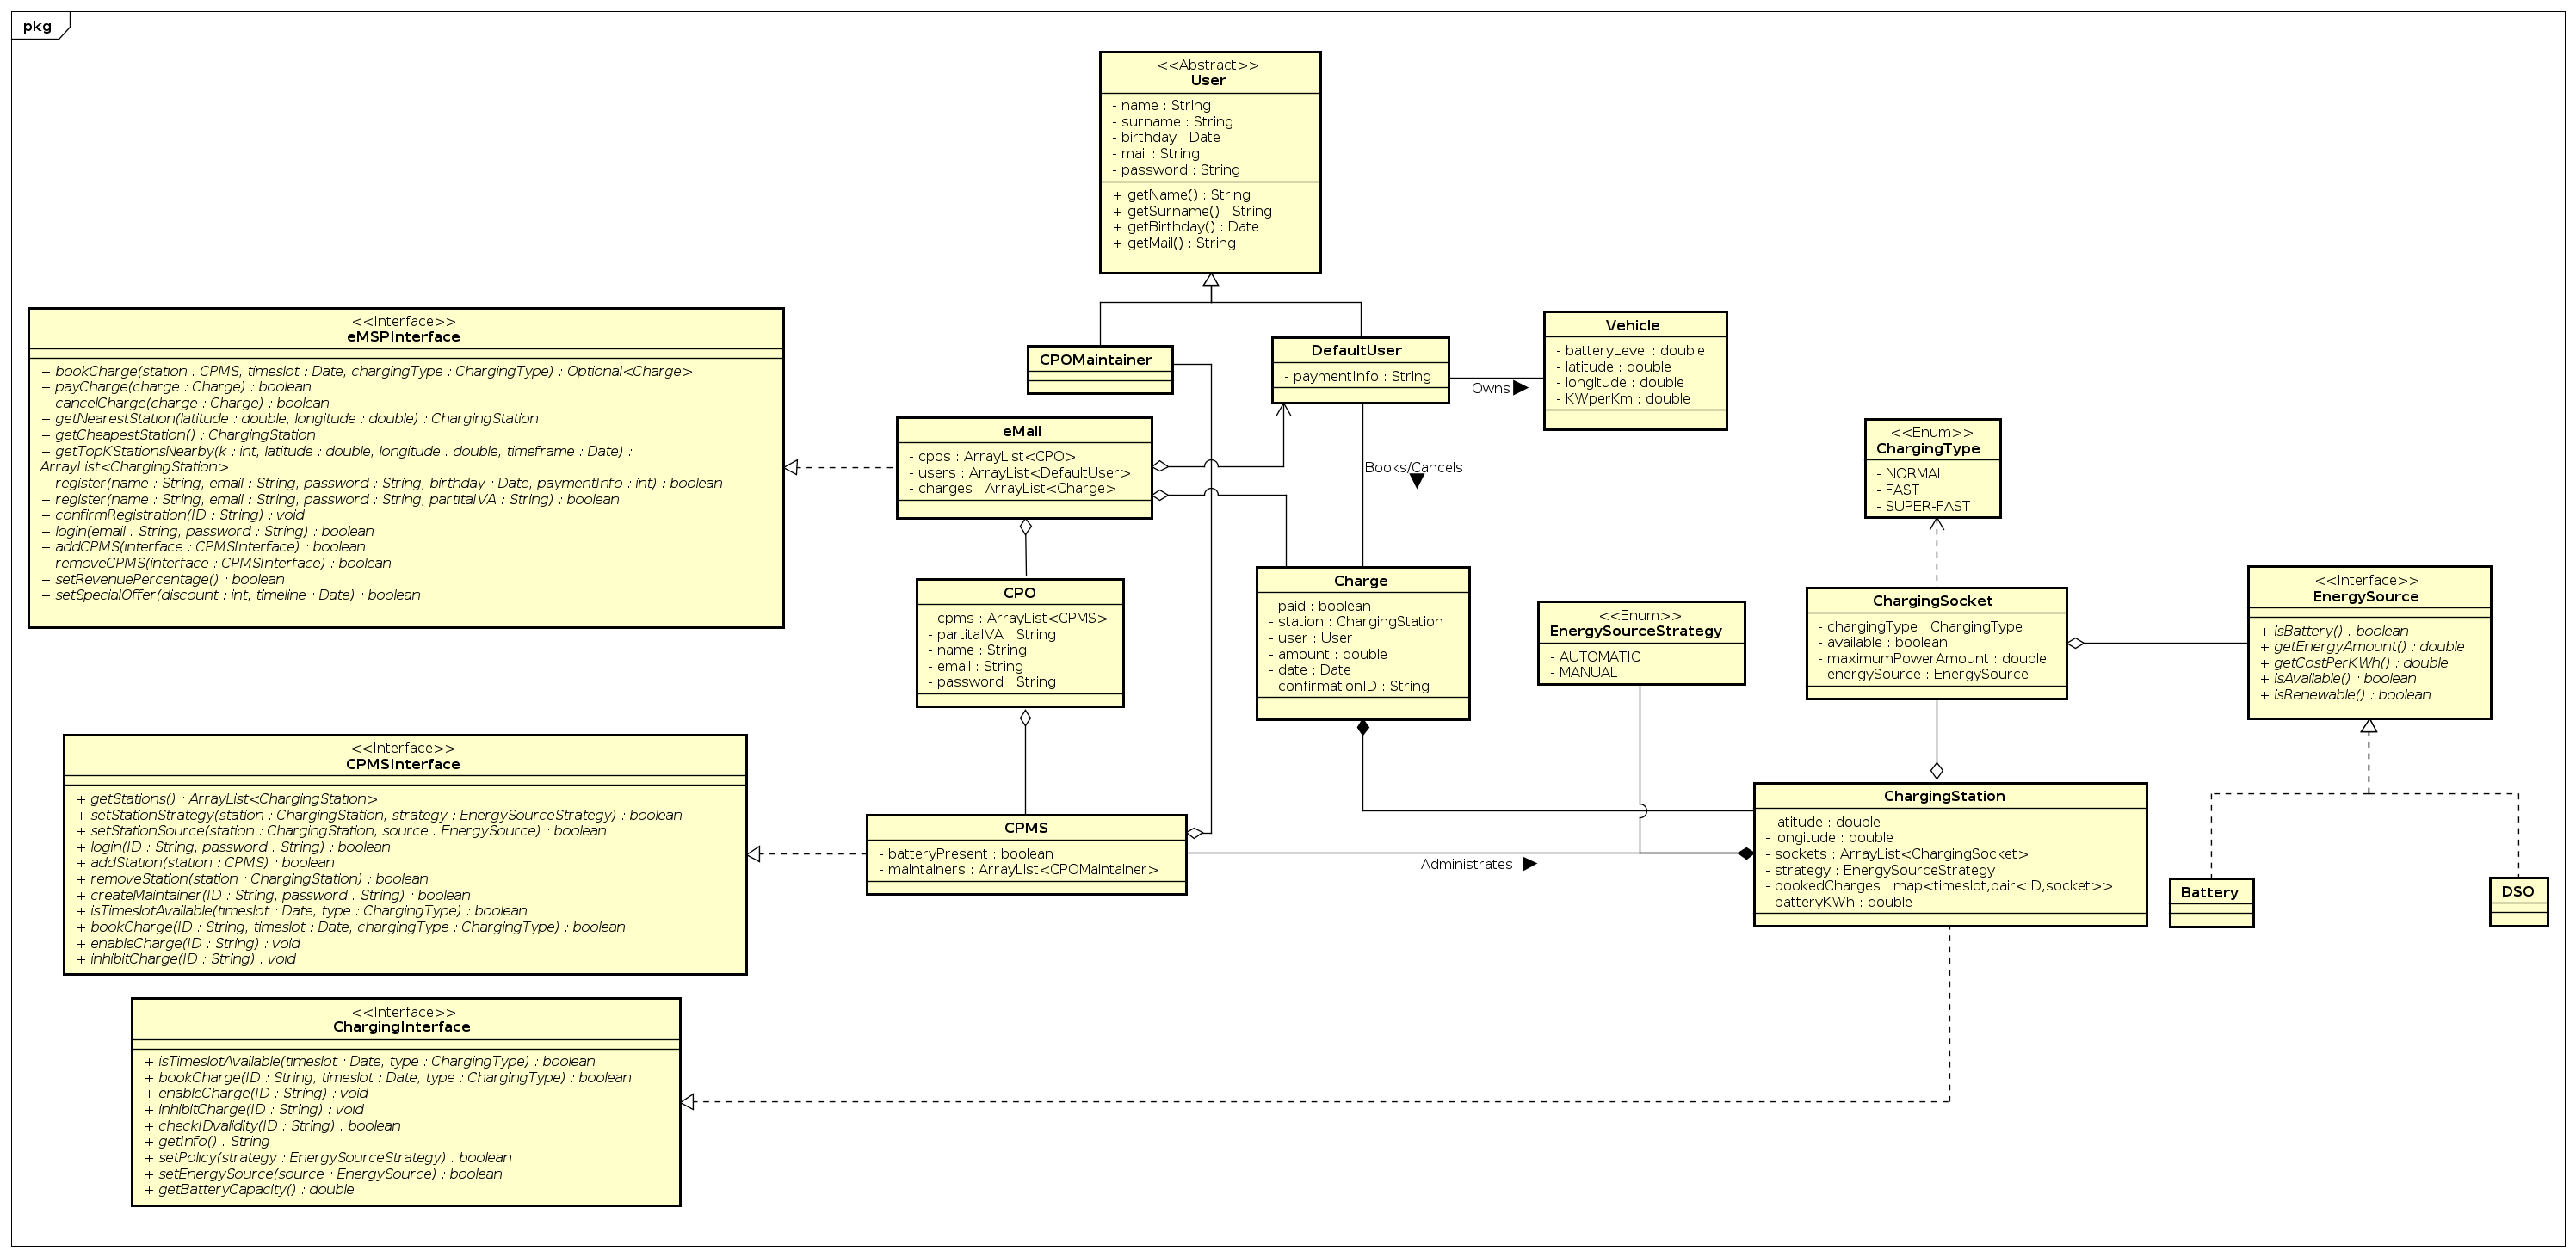
\includegraphics[keepaspectratio, width=16cm]{UML.png}
            \caption{UML}
      \end{center}
\end{figure}

\subsection{Product functions}
In the following subsections the functions of each subsystem are described.

\subsubsection{\ac{eMSP}}
\paragraph{Accessing the \ac{eMSP}}
In order to have features with the usage of personal data (like payment method) the system needs authentication. So a registration and login process is present. When registering it's required to give the system Name, Surname, birthday, e-Mail, Password and a Payment Method. For the login, an authentication with e-Mail and password is required.

\paragraph{Performing a charge}
The principal feature of the system is the ability to help the people to plan a charge for their vehicles efficiently. For this, people can see the availability of charging stations and choose where and in which time slot to charge the vehicle.
Also, if a user changes his mind, there is the possibility to delete a previously booked charge with no charge.
When the user arrives in the booked socket of the charging station, he has to insert the pin that the application displays in order to let the charging process begin.
Always through the application, the user is able to pay for the service thanks to the previously setted payment method.
The system also notifies the user when the charging process is completed.

\paragraph{Retrieving informations about charging stations}
Whenever a user selects a charging station, various informations are shown in order to help the user to make a decision on which station to choose. Informations reguard location, price, a parameter on how green the energy provided is, special offers and availability of sockets in the station.

\paragraph{Get suggestions about the recharge of the vehicle}
An additional feature the system offers reguards a proactive suggestion about the recharge of the vehicle. Thanks to the connection of the application with the vehicle and with the electronic calendar, the system is able to suggest to the user where and when to charge the vehicle in order to satisfy certain parameters chosen by the user. These may involve minimizing the cost of the recharge, minimizing the environment impact of our recharge, minimizing the distance from the scheduled appointments.


\subsubsection{\ac{CPMS}}
\paragraph{Accessing the \ac{CPMS} as \ac{CPO}}
In order to manage the \ac{CPMS} an authentication with proper authorization is required. So \acp{CPO} can login to the system with e-Mail and password. The \ac{CPO} has different informations linked to him in the system, like Name, Surname, e-Mail, password, charging stations that he can manage.
\todo[inline]{2FA for CPO? only login so that the registration will be done by the sysadmin (in this case, add this figure in the rest of the document). If not added manually but we accept registration, it should be authorized by a sysadmin or something like that}

\paragraph{Manage the energy source for a charging station}
An authorized \ac{CPO} can manage stations choosing manually how to charge vehicles, so if he wants to use batteries or \ac{DSO}'s energy in base of their cost and environment impact. In base of these decisions, \acp{CPO} can decide the cost of a charge and special offers to increase visibility of the station in order to promote greener solutions.
Whenever the cost of the energy of some \ac{DSO} is parcticulary convenient the \ac{CPO} can also decide to store it in the batteries. If the \ac{CPO} wishes, the \ac{CPMS} can also work in automatic mode, so the system is able to make all the decisions written above.


\subsection{User characteristics}
We consider the following actors in the \ac{eMall} system:
\begin{enumerate}[label=\textbf{A\arabic*}]
      \item \textbf{Unregistered user:} A user that needs to register before accessing all the \ac{eMall} or \ac{CPMS} services;
      \item \textbf{Registered default user:} A user that has access to all the \ac{eMall} features.
            This actor is associated to an electric vehicle and can visualize the nearest stations, book/cancel/pay a charge, visualize the status of a charge and activate the automatic suggestion service based on the agenda;
      \item \textbf{Registered CPO maintainer user:} A user that has access to all the \ac{CPMS} features.
            These features allow the maintainer to configure the \ac{CPMS} depending on the energy source strategy and visualize all charging stations statuses;
\end{enumerate}

\subsection{Assumptions dependencies and constraints}
\subsubsection{Assumptions}
\begin{enumerate}[label=\textbf{DA\arabic*}]
      \item Users insert genuine data in the forms;
      \item Users(Including CPOs) do not use the system with malicious intent;
      \item All the electric vehicles can be charged by all the stations (no incompatibility);
      \item All the user have an active internet and GPS connection always available while using the service;
\end{enumerate}
\subsubsection{Constraint}
\begin{enumerate}[label=\textbf{C\arabic*}]
      \item If a User wants to change the time slot of a charge he is required to cancel and re-book the charge;
\end{enumerate}

\clearpage

%Here we include more details on all aspects in Section 2 if they
%can be useful for the development team.
\section{Specific Requirements}
\subsection{External interfaces requirements}
\subsubsection{User interfaces}
\begin{enumerate}[label=\textbf{R\arabic*}]
    \item The \ac{eMSP} must allow the users to register (providing email, password, payment method and his infos);
    \item The \ac{CPMS} must allow the \acp{CPO} to register (providing email, password, id-station, partita iva, number of possible charging slots);
    \item The system must allow the \acp{CPO} to modify the possible charging slots in their stations;
          % Maybe not useful anymore R4
    \item The system must verify the correctness of the identification data for the \acp{CPO};
    \item The system must allow the user to login;
    \item The system must allow the user to choose a specific station, a timeslot;
    \item The system must notify the user when the charging process is finished via a notification;
    \item The \ac{CPMS} must allow the \acp{CPO} to choose the mode (manual or automatic) of operation
\end{enumerate}
\subsubsection{Hardware interfaces}
\subsubsection{Software interfaces}
\subsubsection{Communication interfaces}

\subsection{Functional requirements}

\begin{enumerate}[label=\textbf{R\arabic*}]
    \item The system must provide information () about the stations nearby;
    \item The system must reserve a position for a user who registered for a charge through the application;
    \item The system mustn't have collisions in the booking of charges; (non si possono registrare più di X user per timeslot sovrapposti)
    \item The system must take the service money from the user payment method after the charging is finished;
\end{enumerate}
\clearpage
\subsubsection{Sequence diagrams}
\todo[inline]{Per quanto riguarda il sistema CPMS, come si "registra" il CPO maintainer?}
Below there are some sequence diagrams to show how the basic actions should be over time.
\begin{figure}[!h]
    \begin{center}
        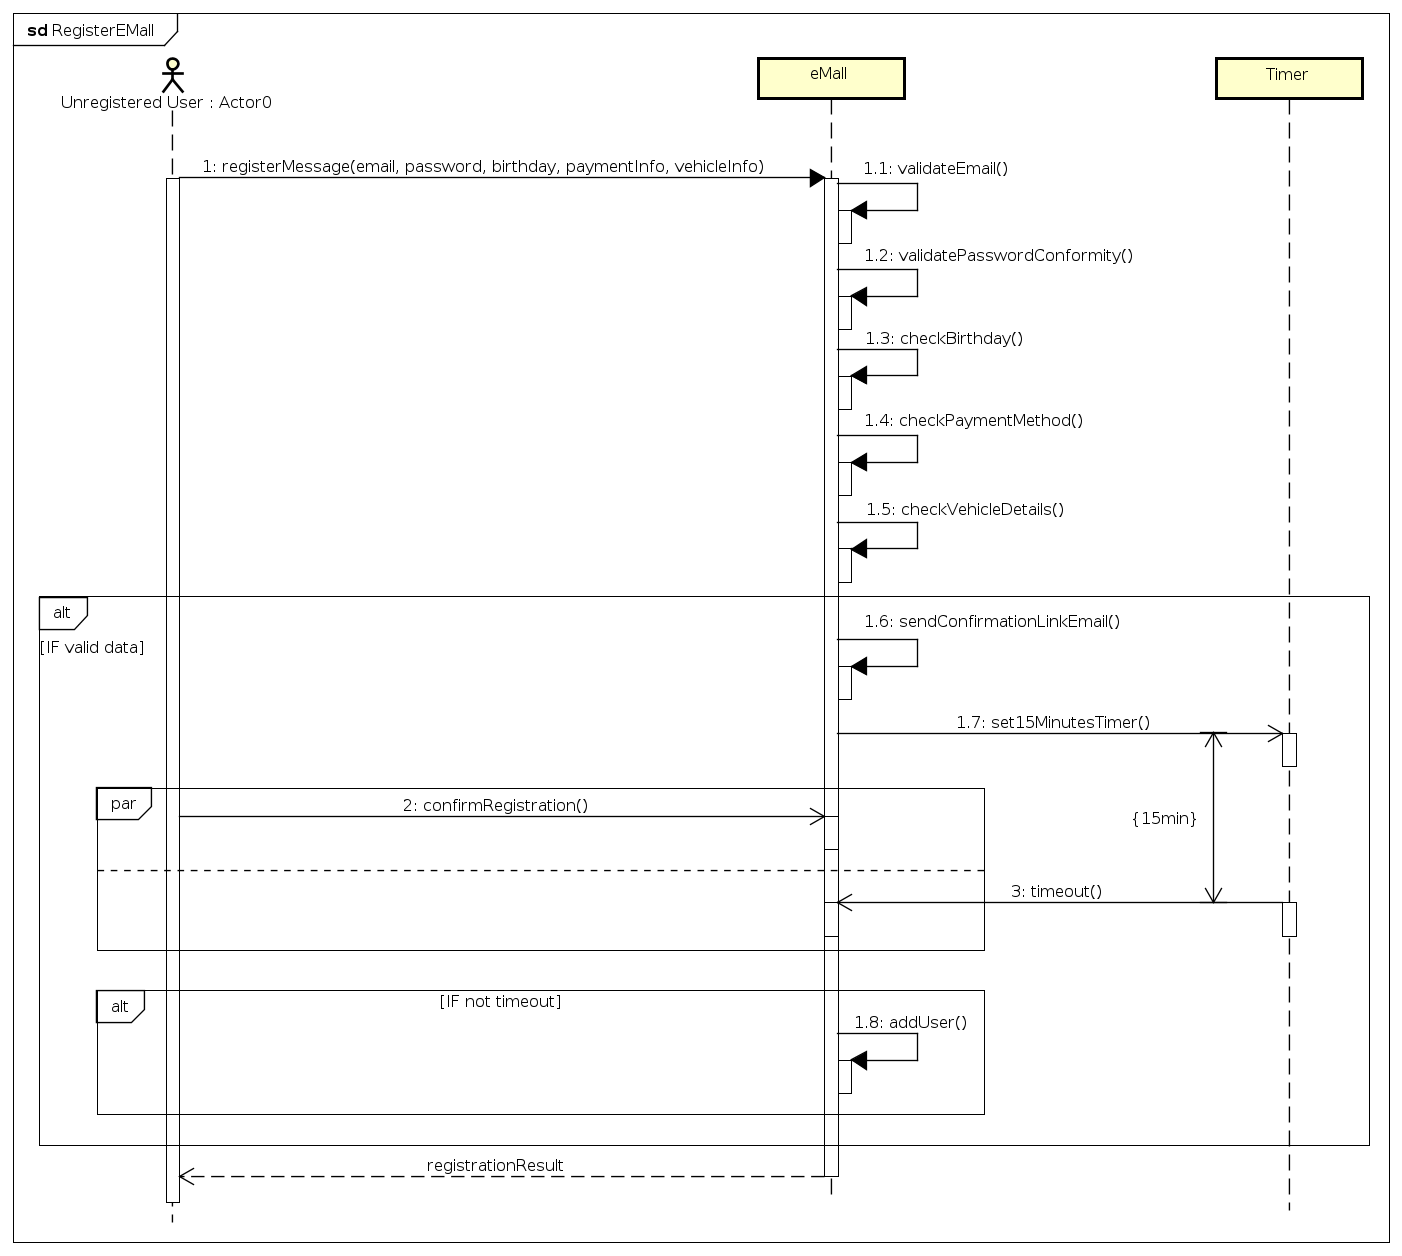
\includegraphics[keepaspectratio, width=16cm]{Sequence/RegisterEMall.png}
        \caption{Registration into \ac{eMall} sequence}
    \end{center}
\end{figure}
\begin{figure}[!h]
    \begin{center}
        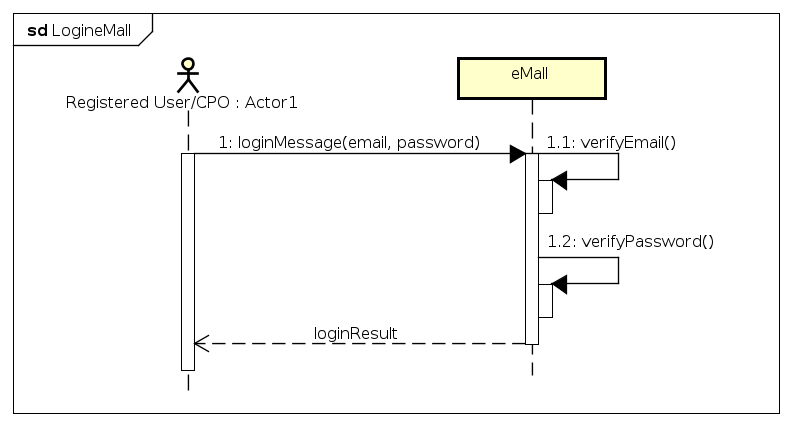
\includegraphics[keepaspectratio, width=16cm]{Sequence/LoginEMall.png}
        \caption{Login into \ac{eMall} sequence}
    \end{center}
\end{figure}
\begin{figure}[!h]
    \begin{center}
        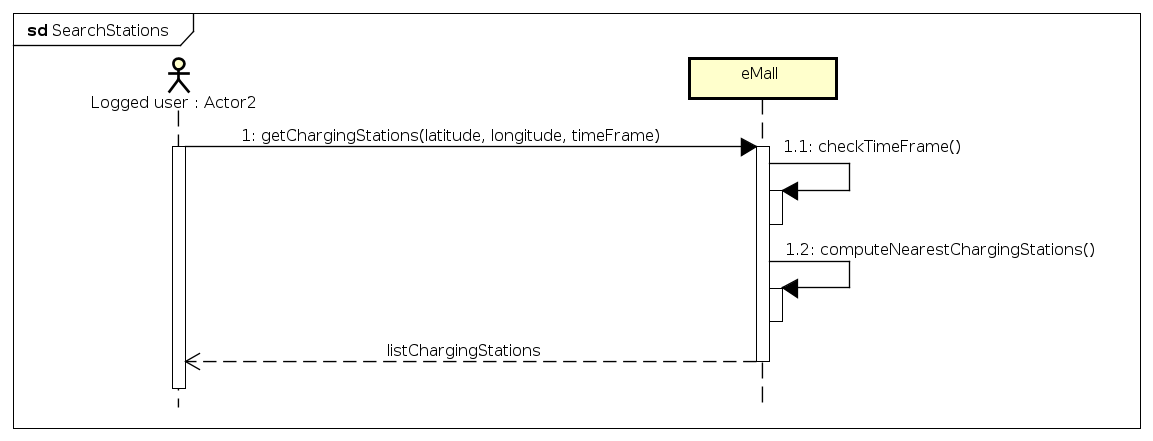
\includegraphics[keepaspectratio, width=16cm]{Sequence/SearchStations.png}
        \caption{Get the nearby charging stations}
    \end{center}
\end{figure}
\begin{figure}[!h]
    \begin{center}
        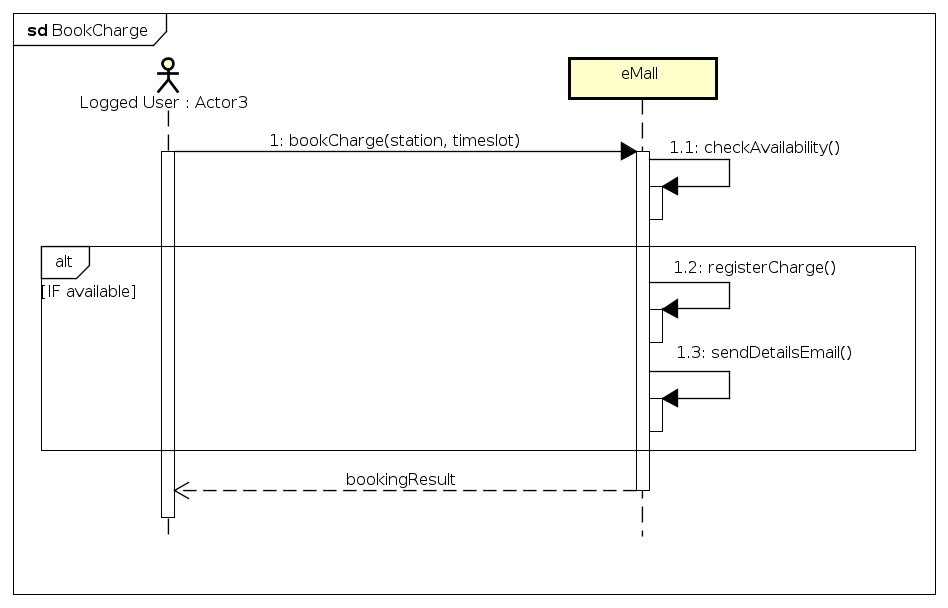
\includegraphics[keepaspectratio, width=16cm]{Sequence/BookCharge.png}
        \caption{Book a charge sequence}
    \end{center}
\end{figure}
\begin{figure}[!h]
    \begin{center}
        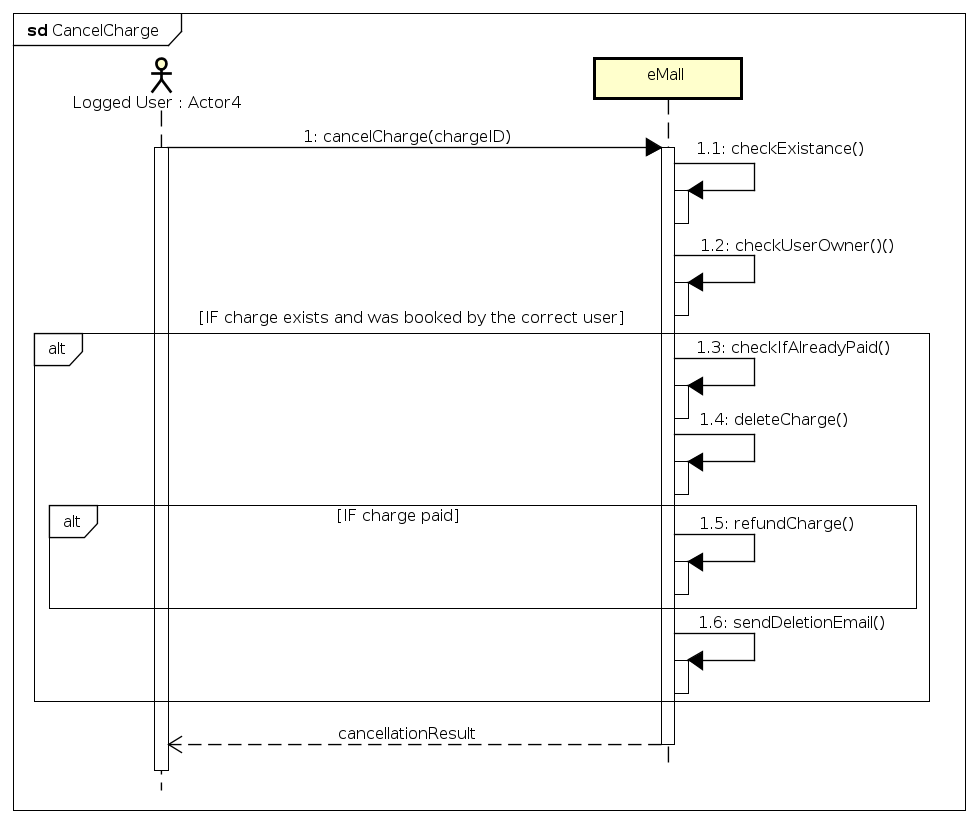
\includegraphics[keepaspectratio, width=16cm]{Sequence/CancelCharge.png}
        \caption{Cancel a charge sequence}
    \end{center}
\end{figure}
\clearpage
%Definition of use case diagrams, use cases and associated sequence/activity diagrams, and mapping on requirements
\subsection{Performance requirements}

\subsection{Design constraints}
\subsubsection{Standards compliance}
\subsubsection{Hardware limitations}
\subsubsection{Other constraints (TODO MAYBE)}

\subsection{Software system attributes}
\subsubsection{Reliability}
\subsubsection{Availability}
\subsubsection{Security}
\subsubsection{Maintainability}
\subsubsection{Portability}
\subsection{Requirements}
\subsubsection{External Interface Requirements}
\clearpage

\section{Formal Analysis Using Alloy}
In this section the system described will be modelled and validated using the AlloyTools framework, the analysis is divided in 4 main parts
\begin{itemize}
    \item Static Analysis
    \item Dynamic Analysis
    \item Assertions
    \item Word Generation
\end{itemize}
For this analysis the following assumption has been considered
\begin{itemize}
    \item The Float type (not defined) represent a decimal number
    \item A CPO can be modelled without being a part of the EMSP
\end{itemize}

\subsection{Static Analysis}
Here the model is created, all the classes are represented by a sig, for the purpose of this analysis only the relational property are considered, so the attribute of a basic type (such as Int,float,boolean,Data etc. etc.) are not considered.
This decision has been taken to simplify the model view and coding, most system that could be used to implement this system already support this type of data, or can be easily implemented and limited in their value ranges.//
As a guideline the type are written only in the declarations in a comment, they are defined by abstract type (not implemented) and their ranges are specified; this types are not considered in the rest of the document.

\begin{verbatim}
module eMall

//-------SIG-----

sig CPO{
cpms: set CPMS}

sig EMSP{
	users: set User,
	charges: set Charge,
	cpos:set CPO
}

sig CPMS{
	stations:set ChargingStation,
	maintainers:set Maintainer
}

abstract sig Person{
	//name: one Str,
	//surname: one Str,
 	//birthday: one Date,
    //mail: one Str,
 	//password: one Str,
} 
sig User extends Person{
	vehicles: set Vehicle
}
sig Maintainer extends Person{}

sig Vehicle{
	//batteryLevel: one Float,
	//KWperKm: one Float,
	location: one Location,
}{ 
//inRange[batteryLevel, 0, 100]
//inRange[KWperKm, 0, 100]
}

sig ChargingStation{
	position:one Location,
	//batteryPresent: one Bool,
	//batteryKWh: one Float,
	sockets: set ChargingSocket,
	strategy: one Strategy
} 
{  
    //batteryPresent.isTrue implies inRange[batteryKWh, 0, 100]
}

sig ChargingSocket{
	chargingType: one ChargingType,
	//available: one Bool,
	//maximumPowerAmount: one Float,
	energySource:one EnergySource
}{ 
    //inRange[maximumPowerAmount, 0, 100]
}

sig Charge{
	//paid: one Bool,
	station: one ChargingStation,
	user: one User
	//amount: one Float,
	//date: one Date
}{
    //amount>0
}

abstract sig Strategy{}
one sig Manual extends Strategy{}
one sig Automatic extends Strategy{}

abstract sig ChargingType{}
one sig SuperFast extends ChargingType{}
one sig Fast extends ChargingType{}
one sig Normal extends ChargingType{}

abstract sig EnergySource{}
sig Battery extends EnergySource{
//capacity: one Float
}{
    //capacity>0
}
sig DSO extends EnergySource{}


//utils types

//sig Date{}

//sig Str{}

//simplified using int
sig Location{  
//	latitude: one Int,   
//	longitude: one Int
}{//  inRange[latitude, -90, 90] and   
//	inRange[longitude, -180, 180]
}

//-------FACTS------

//fact uniqueMailForUser{
//	no disjoint u1,u2: User | u1.mail = u2.mail}

fact uniqueLocationForStation{
	no disjoint s1,s2: ChargingStation | s1.position = s2.position}

fact uniqueCPOForCPMS{
	no disjoint c1,c2: CPO, cp:CPMS | cp in c1.cpms and cp in c2.cpms}

fact uniqueStationForCPMS{
	no disjoint c1,c2: CPMS, s:ChargingStation | s in c1.stations and s in c2.stations}

fact socketOnlyOneStation{
all s:ChargingSocket| s in ChargingStation.sockets
no disjoint c1,c2: ChargingStation, 
s:ChargingSocket|(s in c1.sockets and s in c2.sockets)}

fact noVehicleWithoutUser{
	all v:Vehicle|  v in User.vehicles}

fact noStationWithoutCPMS{
	all s:ChargingStation|  s in CPMS.stations}

fact noUserWithoutEMSP{
	all u:User|  u in EMSP.users}

fact noChargeWithoutEMSP{
	all c:Charge|  c in EMSP.charges}

fact noChargeWithoutUserInTheEMSP{
	all c:Charge| c in EMSP.charges and c.user in EMSP.users
}

fact allChargeAreFromChargingStationInTheSystem{
	all s:Charge.station | s in EMSP.cpos.cpms.stations 
}
fact maintainersMantainStationOfTheSameCPO{
all m:Maintainer, c1,c2:CPO|(not c1=c2 and m in c1.cpms.maintainers) 
implies m not in c2.cpms.maintainers 
}
\end{verbatim}

\subsection{Dynamic Programming}
In this part the major operation are described and run, as a convection letter1 represent the old version (before the execution), while letter0 is the new version after the execution of the predicate.

\subsubsection{User books a charge}
\begin{verbatim}
    pred UserCreatesACharge(e,e1:EMSP,u:User, s:ChargingStation){
        one c:Charge  | u in e1.users and
        c.user=u and c.station=s and  (not (e1 = e)) and  e1.users=e.users and
        e1.cpos=e.cpos and e1.charges=e.charges+c
        }
        run UserCreatesACharge for 3 but exactly 2 EMSP    
\end{verbatim}

\begin{figure}[H]
    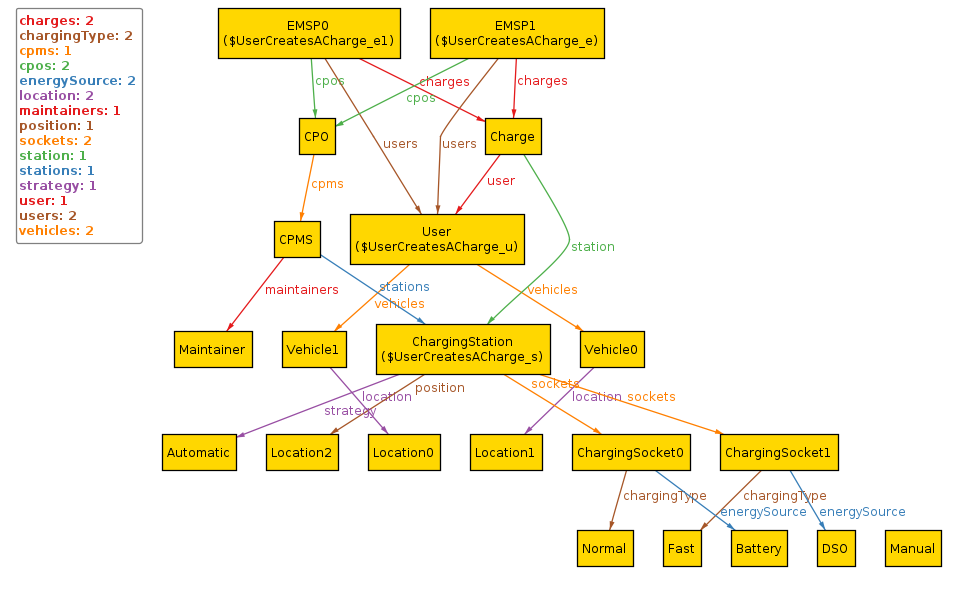
\includegraphics[keepaspectratio, width=16cm]{Alloy/UserCreatesCharge.png}
    \caption{Added Charge}
\end{figure}

\subsubsection{CPO subscribe to EMSP}
\begin{verbatim}
    pred CPOSubscribeItselfToEMSP(e,e1:EMSP,cpo:CPO){
        not (e1 = e)
       e.charges=e1.charges
       e.users= e1.users
       e.cpos=e1.cpos+cpo
       }
       run CPOSubscribeItselfToEMSP for 3 but exactly 2 EMSP, exactly 2 CPO           
\end{verbatim}
\begin{figure}[H]
    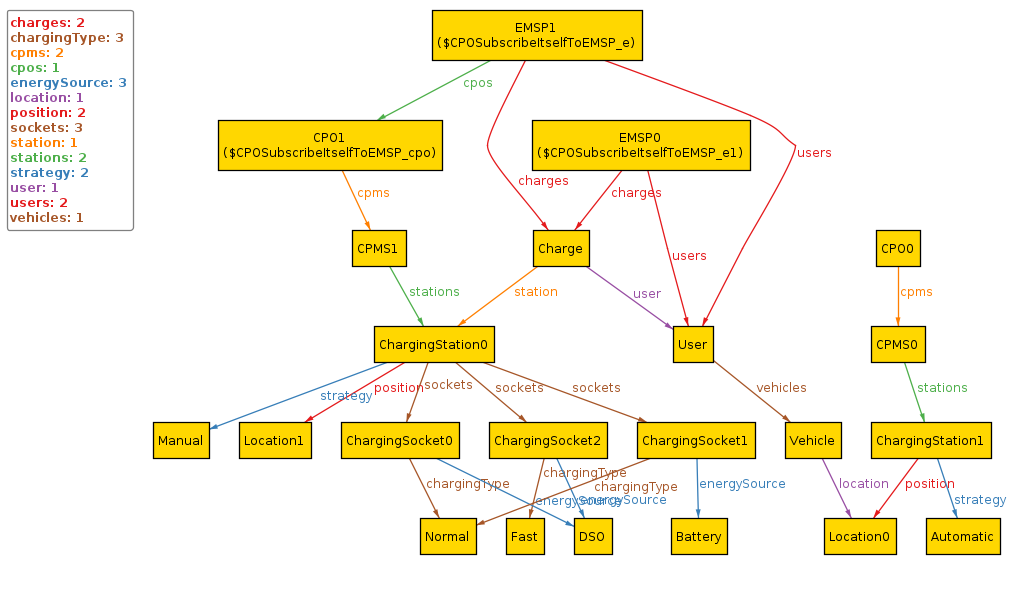
\includegraphics[keepaspectratio, width=16cm]{Alloy/CpoSubscribetoEMSP.png}
    \caption{CPO subscribed}
\end{figure}

\subsubsection{CPO add CPMS}
\begin{verbatim}
    pred CPOAddCPMS(c,c1:CPO,cp:CPMS){
        not (c1 = c)
       c.cpms=c1.cpms+cp
       }
       run CPOAddCPMS for 3 but exactly 2 CPO, exactly 2 CPMS    
\end{verbatim}
\begin{figure}[H]
    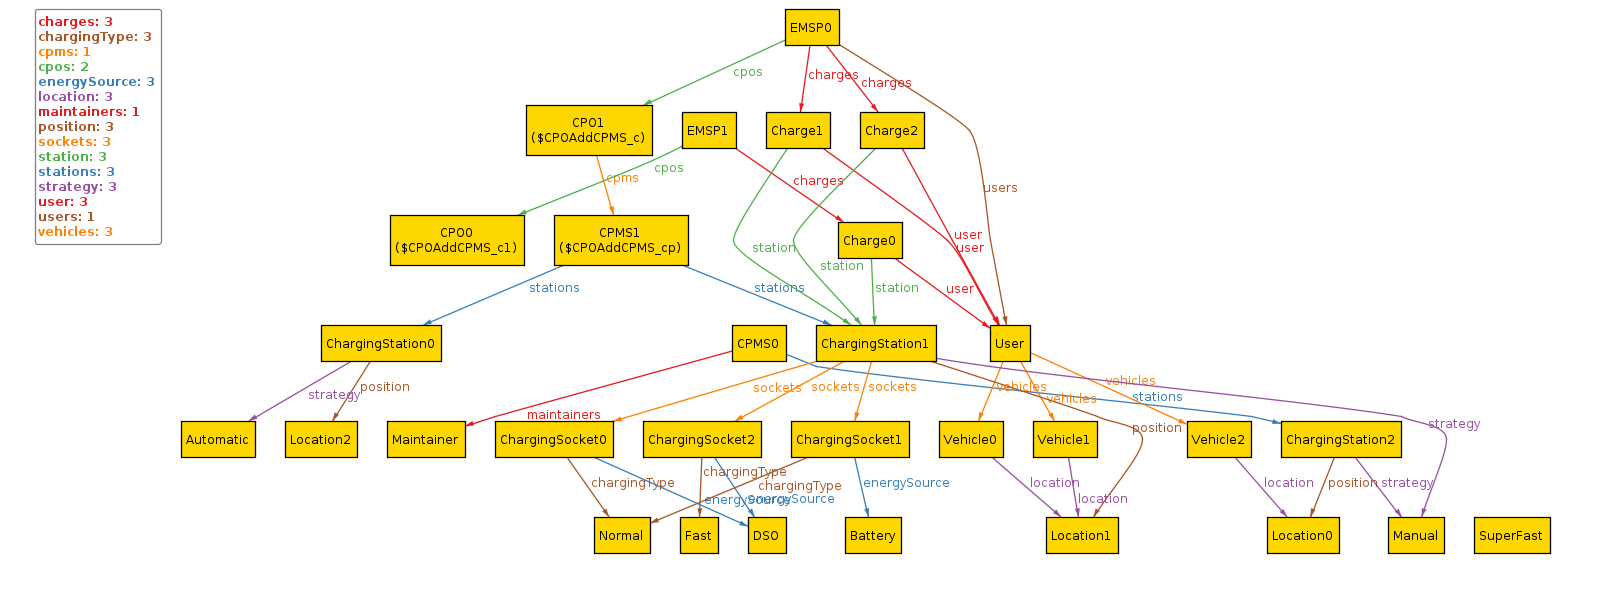
\includegraphics[keepaspectratio, width=16cm]{Alloy/CPOAddCPMS.png}
    \caption{Added CPMS}
\end{figure}

\subsubsection{CPO add mantainer to CPMS}
\begin{verbatim}
    pred CPOAddMantainerToCPMS(c:CPO,cp,cp1:CPMS,m:Maintainer){
        not (cp = cp1)
        cp1 in c.cpms
        cp in c.cpms
        cp.stations=cp1.stations
        cp.maintainers=cp1.maintainers+m
       }
       run CPOAddMantainerToCPMS for 3 but exactly 2 CPMS    
\end{verbatim}
\begin{figure}[H]
    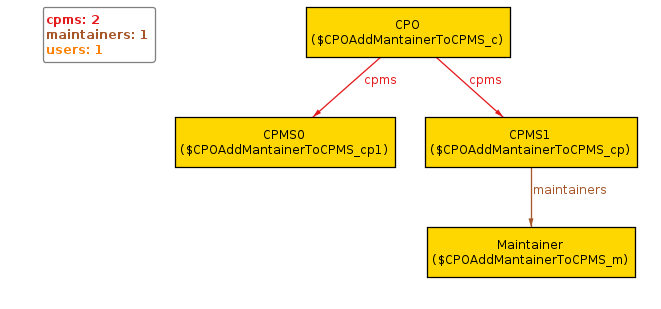
\includegraphics[keepaspectratio, width=16cm]{Alloy/CPoAddMaintainer.png}
    \caption{Added Maintainer}
\end{figure}

\subsubsection{CPO add station to CPMS}
\begin{verbatim}
    pred CPOAddStationToCPMS(c:CPO,cp,cp1:CPMS,s:ChargingStation){
        not (cp = cp1)
        cp1 in c.cpms
        cp in c.cpms
        cp.maintainers = cp1.maintainers
        cp.stations=cp1.stations+s
       }
       run CPOAddStationToCPMS for 3 but exactly 2 CPO    
\end{verbatim}
\begin{figure}[H]
    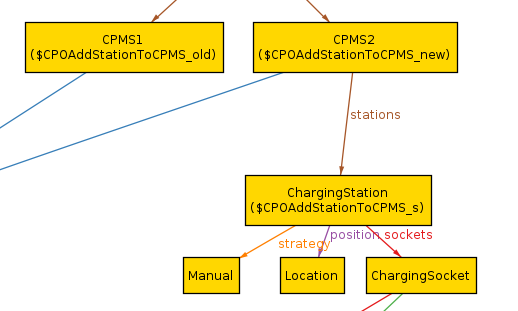
\includegraphics[keepaspectratio, width=16cm]{Alloy/CpoAddStation.png}
    \caption{Added Station}
\end{figure}

\subsubsection{CPO add socket to station}
The following code does not solve, for a limitation of the language,because as a fact a socket can exist only in one station; this is due of the Add patter (s=new station, s1=old station) as for now this pred is never run but supposed as consistent

\begin{verbatim}
    pred CPOAddSocketToStation(c:CPO,cp:CPMS, s,s1:ChargingStation,sk:ChargingSocket){
        not (s = s1)
         cp in c.cpms
         s in cp.stations
         s1 in cp.stations
         s.position=s1.position
         s.strategy=s1.strategy
         s1.sockets=s.sockets+sk
       }
       run CPOAddSocketToStation for 3 but exactly 2 ChargingStation    
\end{verbatim}

\subsection{Assertions}
Here we check the validity of the model trough the Assert notation.
\begin{verbatim}
    assert uniqueLocationForStationCheck{
 	no disjoint s1,s2: ChargingStation | s1.position = s2.position}
check uniqueLocationForStationCheck for 10

assert uniqueCPOForCPMSCheck{
	no disjoint c1,c2: CPO, cp:CPMS | cp in c1.cpms and cp in c2.cpms}
check uniqueCPOForCPMSCheck  for 10

assert uniqueStationForCPMSCheck{
	no disjoint c1,c2: CPMS, s:ChargingStation | s in c1.stations and s in c2.stations}
check uniqueStationForCPMSCheck for 10

assert socketOnlyOneStationCheck{
   all s:ChargingSocket| s in ChargingStation.sockets
	no disjoint c1,c2: ChargingStation, s:ChargingSocket|(s in c1.sockets and s in c2.sockets)}
check socketOnlyOneStationCheck for 10

assert noVehicleWithoutUserCheck{
	all v:Vehicle|  v in User.vehicles}
check noVehicleWithoutUserCheck for 10

assert noStationWithoutCPMSCheck{
	all s:ChargingStation|  s in CPMS.stations}
check noStationWithoutCPMSCheck for 10

assert noUserWithoutEMSP{
	all u:User|  u in EMSP.users}
check noUserWithoutEMSP for 10

assert noChargeWithoutEMSPCheck{
	all c:Charge|  c in EMSP.charges}
check noChargeWithoutEMSPCheck for 10

assert noChargeWithoutUserInTheEMSP{
	all c:Charge| c in EMSP.charges and c.user in EMSP.users}
check noChargeWithoutUserInTheEMSP for 10

assert allChargeAreFromChargingStationInTheSystemCheck{
	all s:Charge.station | s in EMSP.cpos.cpms.stations }
check allChargeAreFromChargingStationInTheSystemCheck for 10

assert maintainersMantainStationOfTheSameCPO{
	all m:Maintainer, c1,c2:CPO|(not c1=c2 and m in c1.cpms.maintainers) implies m not in c2.cpms.maintainers }
check maintainersMantainStationOfTheSameCPO for 10
\end{verbatim}
Which generate the following output.
\begin{figure}[!h]
    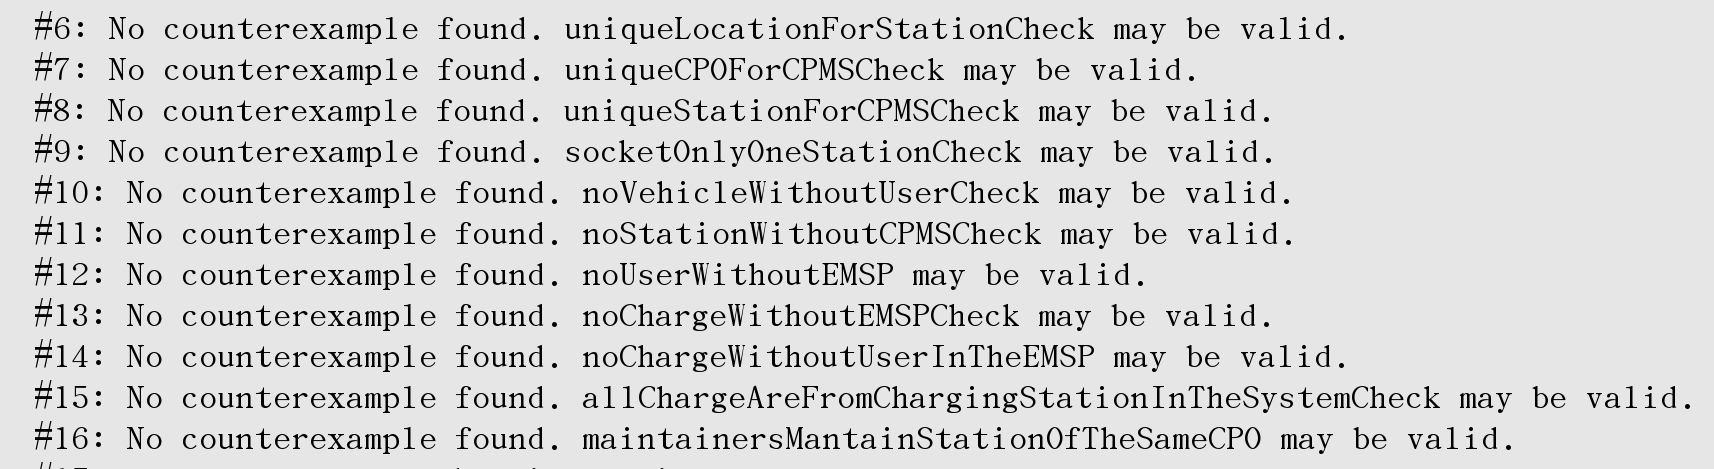
\includegraphics[keepaspectratio, width=16cm]{Alloy/AssertionOutput.png}
    \caption{Assertion output}
\end{figure}
\subsection{Word Generation}
Here is the code of the word generation.
\begin{verbatim}
pred show() {
#EMSP = 1
#CPO>2
#Charge>2
#Vehicle>2
#User>2
}
run show
\end{verbatim}
And the generated word.
\begin{figure}[!h]
    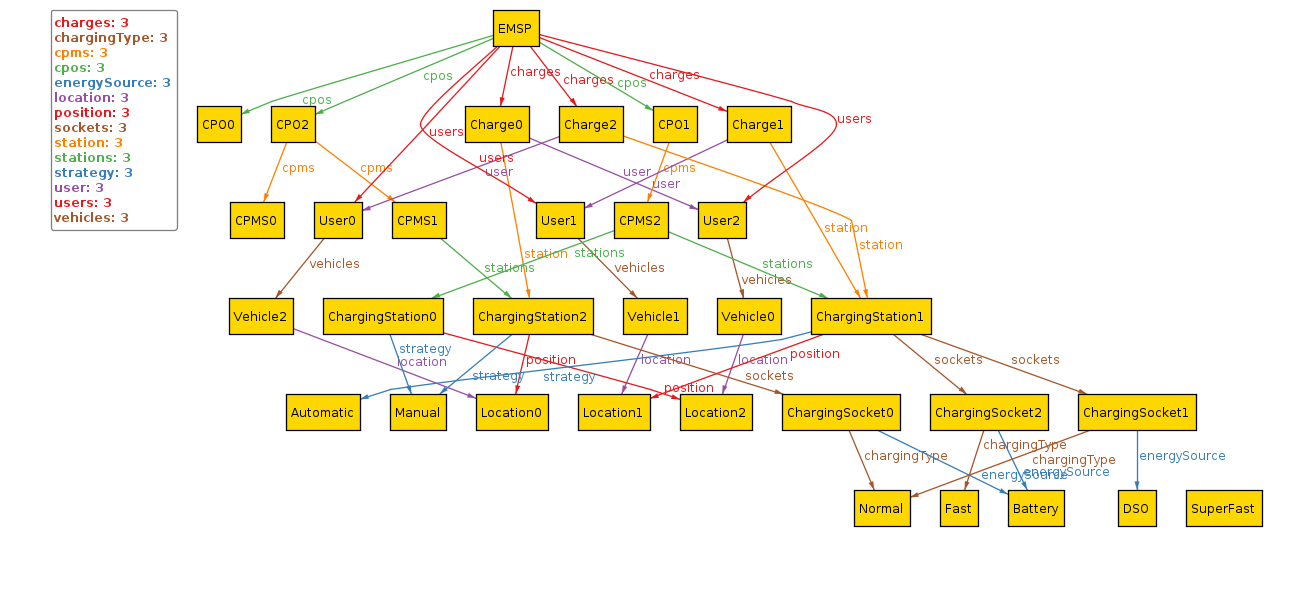
\includegraphics[keepaspectratio, width=16cm]{Alloy/WordResult.png}
    \caption{Generated Word}
\end{figure}
\clearpage

\section{Effort Spent}
\begin{itemize}
    \item 15/11/2022: 15:00 - 18:00 Federico, Emilio, Matteo
    \item 16/11/2022: 08:30 - 10:00 Emilio
    \item 17/11/2022: 21:00 - 23:00 Federico, Emilio, Matteo
    \item 18/11/2022: 10:00 - 12:00 Emilio, Federico
    \item 21/11/2022: 19:00 - 20:00 Matteo
    \item 22/11/2022: 14:30 - 16:00 Matteo
    \item 23/11/2022: 10:30 - 11:30 Matteo
    \item 24/11/2022: 21:30 - 22:30 Matteo, Federico
    \item 25/11/2022: 09:00 - 09:30 Federico
    \item 25/11/2022: 19:00 - 19:30 Matteo
    \item 26/11/2022: 08:30 - 09:00 Federico
    \item 26/11/2022: 16:00 - 17:00 Federico, Emilio, Matteo
    \item 28/11/2022: 08:30 - 09:00 Federico
    \item 28/11/2022: 10:00 - 12:00 Emilio
    \item 30/11/2022: 22:00 - 23:00 Emilio
    \item 28/11/2022: 08:00 - 08:30 Federico
    \item 01/12/2022: 16:00 - 17:30 Matteo
    \item 01/12/2022: 20:30 - 21:30 Emilio
    \item 01/12/2022: 21:30 - 23:00 Federico, Emilio, Matteo
    \item 04/12/2022: 19:00 - 20:00 Emilio
    \item 05/12/2022: 09:00 - 09:30 Federico
    \item 05/12/2022: 11:00 - 11:45 Emilio
    \item 05/12/2022: 15:00 - 16:30 Matteo
    \item 05/12/2022: 19:15 - 19:50 Emilio
    \item 06/12/2022: 15:30 - 17:00 Emilio, Matteo
    \item 07/12/2022: 14:00 - 15:00 Matteo
    \item 10/12/2022: 20:00 - 20:30 Matteo
    \item 11/12/2022: 10:30 - 12:00 Federico
    \item 11/12/2022: 15:10 - 16:40 Matteo
    \item 12/12/2022: 10:00 - 12:00 Emilio
    \item 12/12/2022: 10:30 - 12:00 Emilio
    \item 12/12/2022: 12:30 - 13:00 Matteo
    \item 12/12/2022: 15:00 - 16:30 Federico, Emilio, Matteo
    \item 12/12/2022: 17:30 - 18:30 Emilio
    \item 12/12/2022: 19:00 - 19:30 Matteo
    \item 12/12/2022: 22:00 - 23:00 Federico
    \item 13/12/2022: 15:15 - 17:00 Emilio, Matteo
    \item 15/12/2022: 10:00 - 16:00 Federico
    \item 17/12/2022: 17:00 - 01:00 Federico
    \item 17/12/2022: 10:30 - 12:00 Federico, Emilio, Matteo
    \item 17/12/2022: 21:00 - 22:00 Federico, Emilio, Matteo
    \item 18/12/2022: 09:30 - 11:30 Matteo
    \item 18/12/2022: 09:30 - 12:00 Federico
    \item 18/12/2022: 16:30 - 21:00 Federico
    \item 20/12/2022: 09:00 - 12:30 Federico
    \item 19/12/2022: 09:30 - 11:30 Emilio
    \item 20/12/2022: 14:00 - 15:30 Emilio
    \item 21/12/2022: 10:30 - 11:45 Matteo
    \item 21/12/2022: 10:45 - 12:00 Emilio
    \item 21/12/2022: 12:00 - 22:00 Federico
    \item 21/12/2022: 14:00 - 15:40 Emilio
    \item 21/12/2022: 17:15 - 18:15 Matteo
    \item 21/12/2022: 17:20 - 18:10 Emilio
    \item 22/12/2022: 16:30 - 18:30 Emilio
    \item 22/12/2022: 22:30 - 01:30 Emilio
\end{itemize}

\section{References}
\begin{itemize}
    \item \textbf{\ac{RACS} and \ac{RAPS}}: \url{https://arxiv.org/pdf/cs/9912010.pdf}
\end{itemize}
\clearpage

\end{document}
